%\input{Preambulum}

\begin{figure}[t!]
\centering

\begin{subfigure}{\textwidth}
\caption{Graphs with pair constraints ($G_1$--$G_{31}$ plus one pair of nodes, Figure~\ref{Fig1})}
\label{Fig6a}

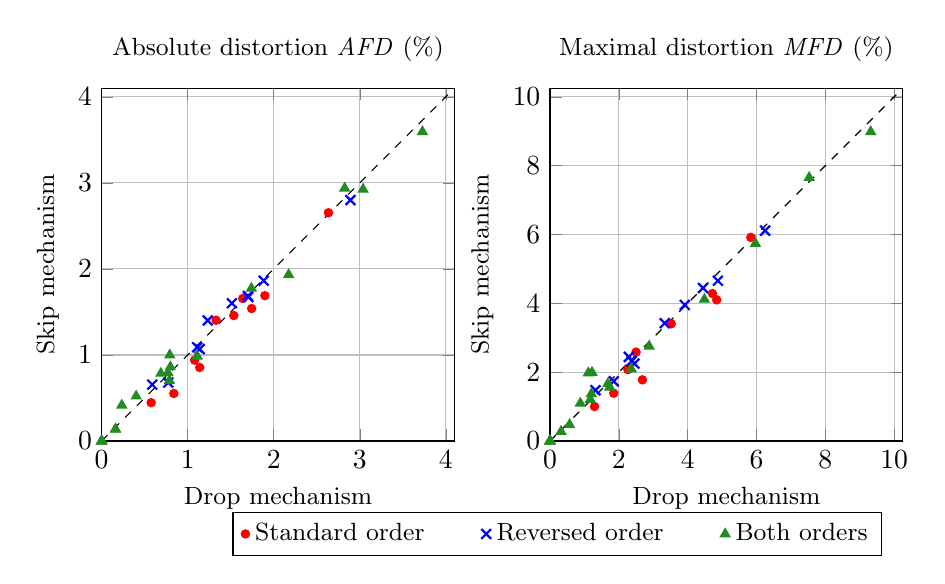
\begin{tikzpicture}
\begin{axis}[
name = axis1,
title = {Absolute distortion $\mathit{AFD}$ (\%)},
title style = {font=\small},
xlabel = Drop mechanism,
x label style = {font=\small},
ylabel = Skip mechanism,
y label style = {font=\small},
width = 0.5\textwidth,
height = 0.5\textwidth,
nodes near coords,
xmajorgrids = true,
ymajorgrids = true,
xmin = 0,
xmax = 4.1,
ymin = 0,
ymax = 4.1,
]
\addplot [scatter,red,only marks,mark size=1.5pt,point meta=explicit symbolic] coordinates {
(0.575196408529747,0.445566778900112)
(0.838779956427026,0.552287581699346)
(1.32988380537401,1.40359477124183)
(1.08035371011149,0.939830834294502)
(1.74300044091711,1.53968253968254)
(1.89670138888888,1.68923611111111)
(1.63966049382716,1.65625)
(2.63558201058201,2.65277777777778)
(1.13960113960113,0.854700854700854)
(1.5354938271605,1.45833333333333)
};
\addplot [scatter,blue,only marks,mark=x,mark size=2.5pt,thick,point meta=explicit symbolic] coordinates {
(0.588056490834269,0.655443322109989)
(0.774328249818459,0.679738562091503)
(1.23275236020334,1.40114379084967)
(1.10985625186893,1.08852364475202)
(1.70345568783069,1.67162698412698)
(1.69959766313932,1.68576388888889)
(1.51331018518517,1.60069444444444)
(2.89021164021163,2.79960317460317)
(1.13960113960115,1.06837606837607)
(1.8827160493827,1.86342592592592)
};
\addplot [scatter,ForestGreen,only marks,mark=triangle*,mark size=2pt,point meta=explicit symbolic] coordinates {
(0,0)
(0.234250398724091,0.416267942583732)
(0,0)
(0.400891632373112,0.521604938271604)
(0.791340218423561,0.999287749287749)
(0.787037037037033,0.702614379084968)
(1.11082444673777,0.985552115583075)
(0.769562454611469,0.793300653594771)
(0,0)
(0,0)
(0.160108024691384,0.13888888888889)
(2.1728570426487,1.93292297979798)
(2.82366071428573,2.93799603174603)
(3.03780864197532,2.925)
(3.72727272727272,3.59393939393939)
(0.798611111111113,0.861111111111111)
(1.73960170487948,1.77380952380953)
(0.6878306878307,0.785714285714285)
(0,0)
(0.162337662337664,0.135281385281388)
(0,0)
};
% Zero line
\draw [black,dashed] (rel axis cs:0,0) -- (rel axis cs:1,1);
\end{axis}

\begin{axis}[
at = {(axis1.south east)},
xshift = 0.1\textwidth,
title = {Maximal distortion $\mathit{MFD}$ (\%)},
title style = {font=\small},
xlabel = Drop mechanism,
x label style = {font=\small},
ylabel = Skip mechanism,
y label style = {font=\small},
width = 0.5\textwidth,
height = 0.5\textwidth,
nodes near coords,
xmajorgrids = true,
ymajorgrids = true,
xmin = 0,
xmax = 10.25,
ymin = 0,
ymax = 10.25,
legend style = {font=\small,at={(-0.9,-0.2)},anchor=north west,legend columns=3},
legend entries = {Standard order$\qquad$,Reversed order$\qquad$,Both orders}
]
\addplot [scatter,red,only marks,mark size=1.5pt,point meta=explicit symbolic] coordinates {
(1.2941919191919,1.00252525252525)
(2.68518518518526,1.77777777777778)
(3.51273148148151,3.41666666666667)
(2.26307189542483,2.07516339869281)
(4.84347442680776,4.10119047619048)
(4.71781305114639,4.28571428571429)
(2.50000000000009,2.58333333333334)
(5.83333333333331,5.91666666666667)
(1.85185185185186,1.38888888888889)
(3.5185185185185,3.40277777777778)
};
\addplot [scatter,blue,only marks,mark=x,mark size=2.5pt,thick,point meta=explicit symbolic] coordinates {
(1.32312710437707,1.47474747474748)
(2.45370370370376,2.25)
(3.33333333333335,3.42361111111111)
(2.37495461147419,2.32516339869281)
(4.87819664903005,4.65674603174603)
(3.91644620811283,3.95238095238095)
(2.29166666666673,2.44444444444444)
(6.24999999999996,6.11111111111111)
(1.85185185185188,1.73611111111111)
(4.44444444444441,4.44444444444444)
};
\addplot [scatter,ForestGreen,only marks,mark=triangle*,mark size=2pt,point meta=explicit symbolic] coordinates {
(0,0)
(1.11268939393942,1.97727272727273)
(0,0)
(1.17206790123456,1.20833333333333)
(1.22188093542263,1.99252136752137)
(1.6820987654321,1.66666666666667)
(2.36050194931776,2.09429824561403)
(1.73032407407407,1.5625)
(0,0)
(0,0)
(0.320216049382771,0.277777777777777)
(4.48565516273854,4.11489898989899)
(7.52976190476193,7.65476190476191)
(5.96836419753091,5.73611111111111)
(9.31818181818183,8.98484848484848)
(0.879629629629657,1.09722222222223)
(2.88111772486773,2.75496031746032)
(1.2037037037037,1.375)
(0,0)
(0.568181818181798,0.473484848484848)
(0,0)
};
% Zero line
\draw [black,dashed] (rel axis cs:0,0) -- (rel axis cs:1,1);
\end{axis}
\end{tikzpicture}
\end{subfigure}

\vspace{0.25cm}
\begin{subfigure}{\textwidth}
\caption{Graphs without pair constraints ($H_1$--$H_{31}$ plus one pair of nodes, Figure~\ref{Fig2})}
\label{Fig6b}

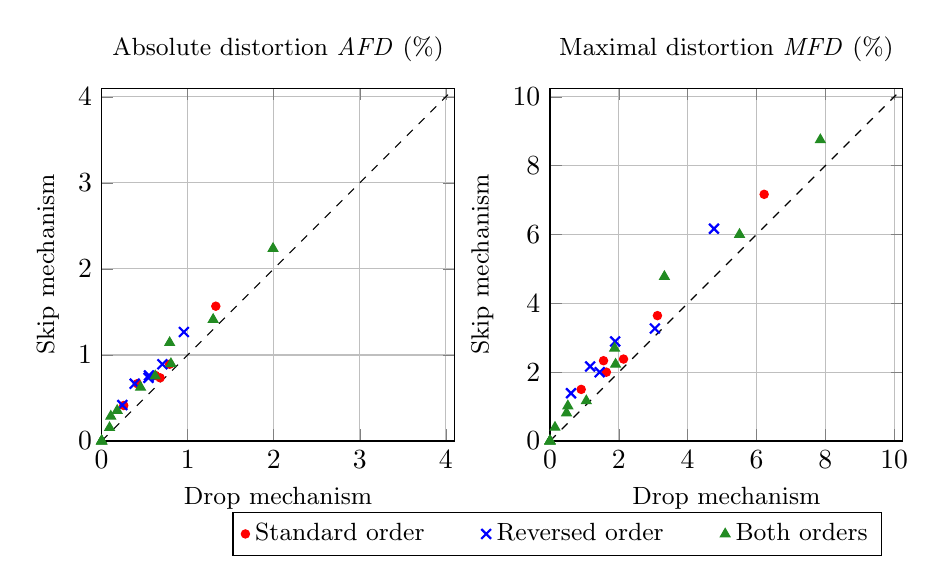
\begin{tikzpicture}
\begin{axis}[
name = axis1,
title = {Absolute distortion $\mathit{AFD}$ (\%)},
title style = {font=\small},
xlabel = Drop mechanism,
x label style = {font=\small},
ylabel = Skip mechanism,
y label style = {font=\small},
width = 0.5\textwidth,
height = 0.5\textwidth,
nodes near coords,
xmajorgrids = true,
ymajorgrids = true,
xmin = 0,
xmax = 4.1,
ymin = 0,
ymax = 4.1,
]
\addplot [scatter,red,only marks,mark size=1.5pt,point meta=explicit symbolic] coordinates {
(0.414141414141424,0.666666666666666)
(0.256613756613751,0.412698412698412)
(0.624338624338617,0.761904761904762)
(0.789566508864749,0.892230576441104)
(0.679138321995467,0.734693877551021)
(1.32638888888888,1.56666666666667)
};
\addplot [scatter,blue,only marks,mark=x,mark size=2.5pt,thick,point meta=explicit symbolic] coordinates {
(0.383838383838391,0.666666666666666)
(0.240740740740732,0.417989417989418)
(0.550264550264545,0.761904761904762)
(0.705096073517122,0.892230576441103)
(0.544217687074826,0.734693877551021)
(0.955555555555559,1.26666666666667)
};
\addplot [scatter,ForestGreen,only marks,mark=triangle*,mark size=2pt,point meta=explicit symbolic] coordinates {
(0,0)
(0,0)
(0.180602006688967,0.354515050167223)
(0.106060606060613,0.287878787878788)
(0.0916442048517484,0.155136268343816)
(0,0)
(0.790123456790121,1.14285714285714)
(0.451929012345677,0.625)
(0,0)
(0.622222222222225,0.755555555555556)
(0.80495219530306,0.898078529657478)
(1.29557007988381,1.41176470588235)
(0,0)
(1.99122807017544,2.23684210526316)
};
% Zero line
\draw [black,dashed] (rel axis cs:0,0) -- (rel axis cs:1,1);
\end{axis}

\begin{axis}[
at = {(axis1.south east)},
xshift = 0.1\textwidth,
title = {Maximal distortion $\mathit{MFD}$ (\%)},
title style = {font=\small},
xlabel = Drop mechanism,
x label style = {font=\small},
ylabel = Skip mechanism,
y label style = {font=\small},
width = 0.5\textwidth,
height = 0.5\textwidth,
nodes near coords,
xmajorgrids = true,
ymajorgrids = true,
xmin = 0,
xmax = 10.25,
ymin = 0,
ymax = 10.25,
legend style = {font=\small,at={(-0.9,-0.2)},anchor=north west,legend columns=3},
legend entries = {Standard order$\qquad$,Reversed order$\qquad$,Both orders}
]
\addplot [scatter,red,only marks,mark size=1.5pt,point meta=explicit symbolic] coordinates {
(1.5555555555556,2.33333333333334)
(0.907407407407429,1.5)
(1.63888888888892,2)
(2.13712522045853,2.38095238095238)
(3.12202380952388,3.64285714285715)
(6.22222222222223,7.16666666666667)
};
\addplot [scatter,blue,only marks,mark=x,mark size=2.5pt,thick,point meta=explicit symbolic] coordinates {
(1.16666666666665,2.16666666666667)
(0.61111111111109,1.38888888888888)
(1.44444444444448,2)
(3.04761904761908,3.26984126984127)
(1.89285714285721,2.89285714285715)
(4.7638888888889,6.16666666666667)
};
\addplot [scatter,ForestGreen,only marks,mark=triangle*,mark size=2pt,point meta=explicit symbolic] coordinates {
(0,0)
(0,0)
(0.51923076923075,1.01923076923077)
(0.145833333333362,0.395833333333334)
(0.48113207547171,0.814465408805032)
(0,0)
(3.32407407407409,4.77777777777778)
(1.87731481481482,2.69444444444444)
(0,0)
(1.05555555555555,1.16666666666667)
(1.90608465608467,2.23015873015873)
(5.50617283950621,6)
(0,0)
(7.85416666666667,8.75)
};
% Zero line
\draw [black,dashed] (rel axis cs:0,0) -- (rel axis cs:1,1);
\end{axis}
\end{tikzpicture}
\end{subfigure}

\caption{Fairness distortions of the Drop and Skip mechanisms \\ for selected balanced bipartite graphs with 10 nodes}
\label{Fig6}
\end{figure}

%\end{document}